%&pdflatex
\documentclass[11pt, twocolumn]{article}
\usepackage{setspace}
\usepackage{microtype}
\usepackage{fullpage}
\usepackage{enumitem}
\usepackage{graphicx}
\usepackage{titlesec}
\usepackage{lipsum}
\usepackage{float}

\hbadness=99999  % or any number >=10000

\graphicspath{{../figures/}}

\titleformat{\section}{\normalfont\scshape}{\thesection}{1em}{}
\titleformat{\subsubsection}{\normalfont\scshape}{\thesection}{1em}{}

\begin{document}

\title{Molecular Dynamics Simulation of the D102A Variant of Chymotrypsin}
\author{David Li, Patrick Fleming}
\date{\today}
\maketitle

\section{Introduction}
Almost one third of all proteases can be classified as serine proteases \cite{hedstrom02}.
These protiens are named for the nucleophilic Ser residue at the active site.
Serine proteases fall into two broad categories based on their structure
-- chymotrypsin-like (trypsin-like) or subtilisin-like \cite{madala10}.
Chymotrypsin-like proteases are the most abundant in nature and can be found in
eukaryotes, prokaryotes, archae, and viruses. They are involved in many critical
physiological processes, such as hemostasis, apoptosis, digestion, and reproduction
\cite{hedstrom02}.

In order to hydrolyze a peptide bond, these well-studied enzymes must overcome
three major mechanistic barriers: (1) amide bonds are extremely stable due to electron
donation from the amide nitrogen to the carbonyl; (2) water is a poor nucleophile
and proteases always activate water via a general base; (3) and amines are poor leaving
groups because proteases protonate the amine prior to expulsion \cite{hedstrom02}.

To overcome these three reaction barriers, serine proteases contain a group of three
residues called the catalytic triad that use hydrogen bonding to increase reaction favorability.
In chymotrypsin, the triad is composed of serine, histidine, and aspartate, and is part of
a larger hydrogen bonding network \cite{hedstrom02}.

% \includegraphics{}

Mutagenesis experiments of catalytic
triad residues show decreased catalytic activity; substitution of Ser195 or His57 with Ala
effectively disables the triad \cite{hedstrom02}. For this project, we hypothesize that
the Asp-His hydrogen bond restrains the conformational flexibility of the His ring so that
it can more strongly hydrogen bond to Ser, thus activating serine for a nucleophilic attack.

To test this, we carried out two all-atom molecular dynamics simulations of two
chymotrypsin series variants: the wild type sequence, and with Asp-102 substituted for
alanine (mutation D102A). This enabled us to determine rotamer distributions of the
His side chain and the time-dependent frequencies of His-Ser bond formations.

\section{Methods}

\lipsum[1-3]

\section{Results}

\begin{figure}[H]
    \centering
        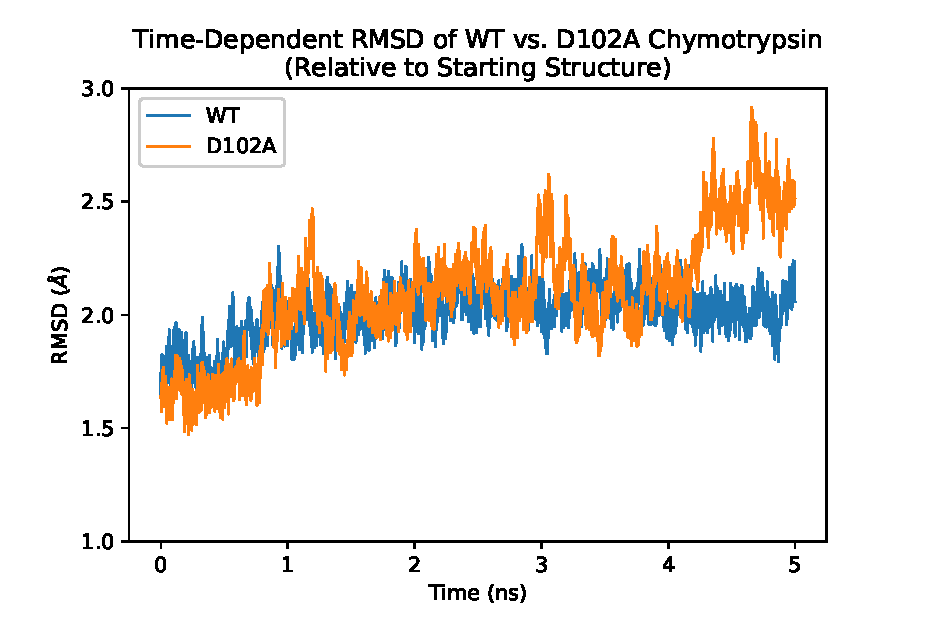
\includegraphics[width=0.49\textwidth]{rmsds.eps}
    \caption{RMSD of wild-type (WT) and D102A simulations}
\end{figure}

\begin{figure}[H]
    \centering
        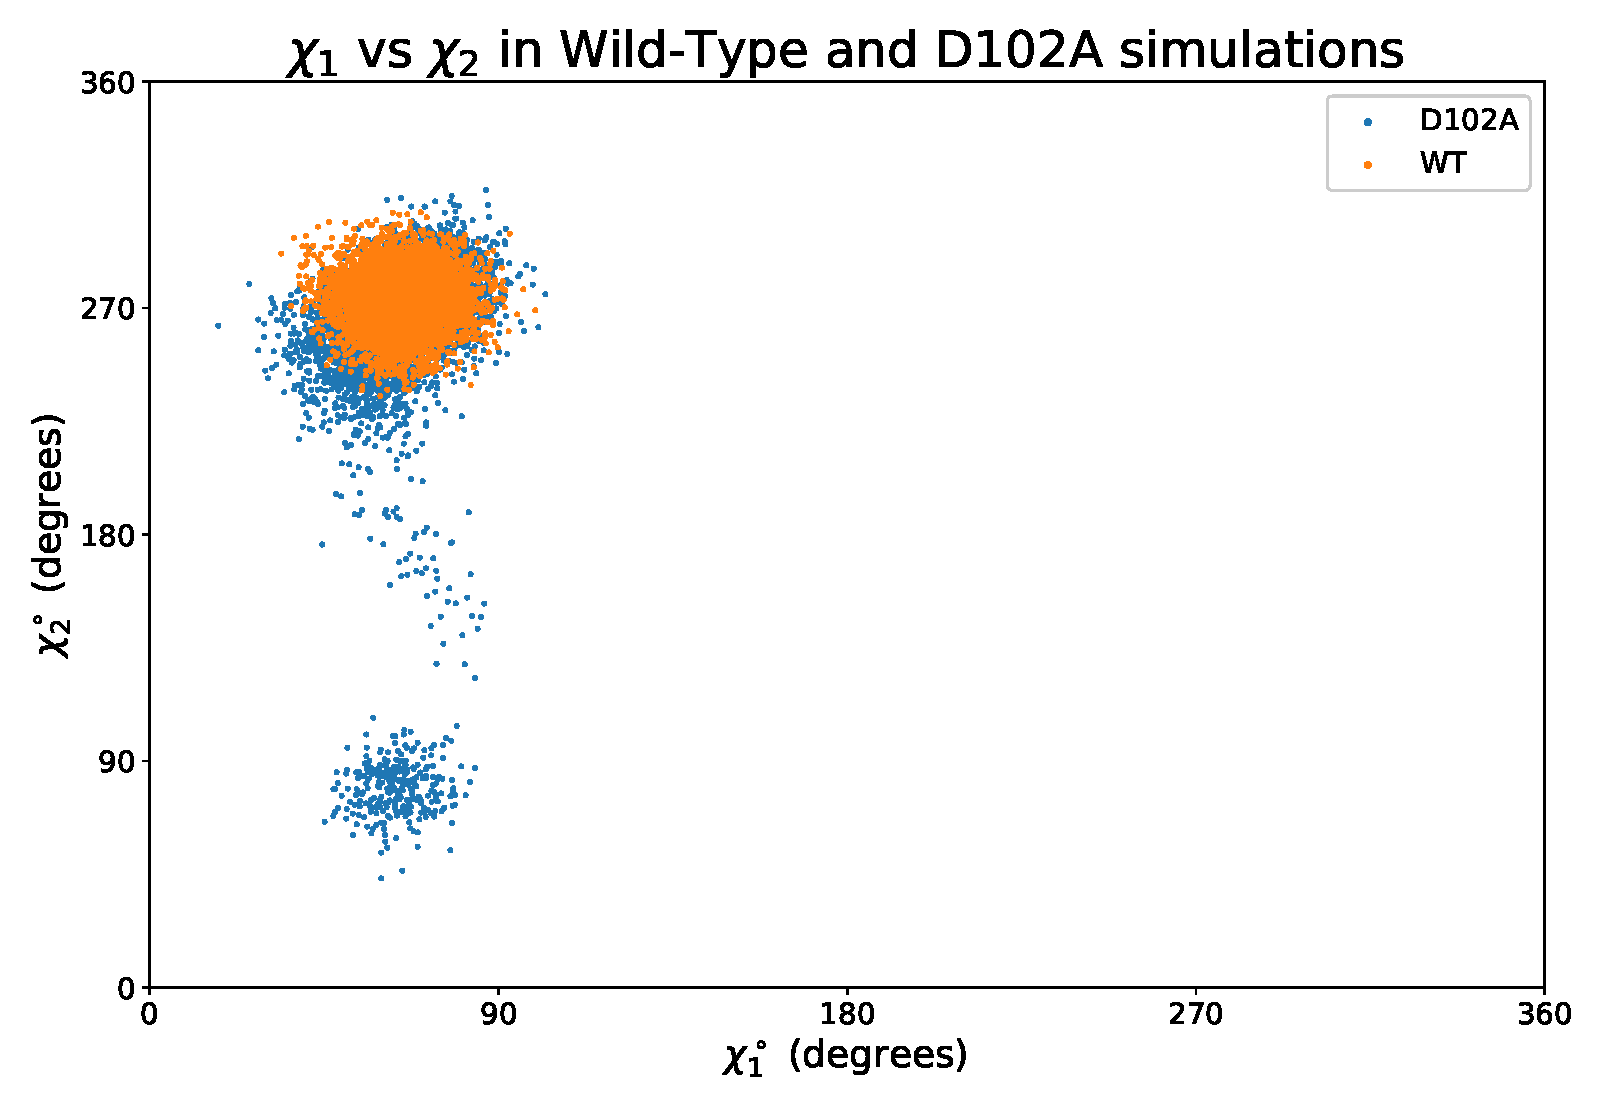
\includegraphics[width=0.49\textwidth]{chi_plot_wt_d102a.eps}
    \caption{}
\end{figure}

\begin{figure}[H]
    \centering
        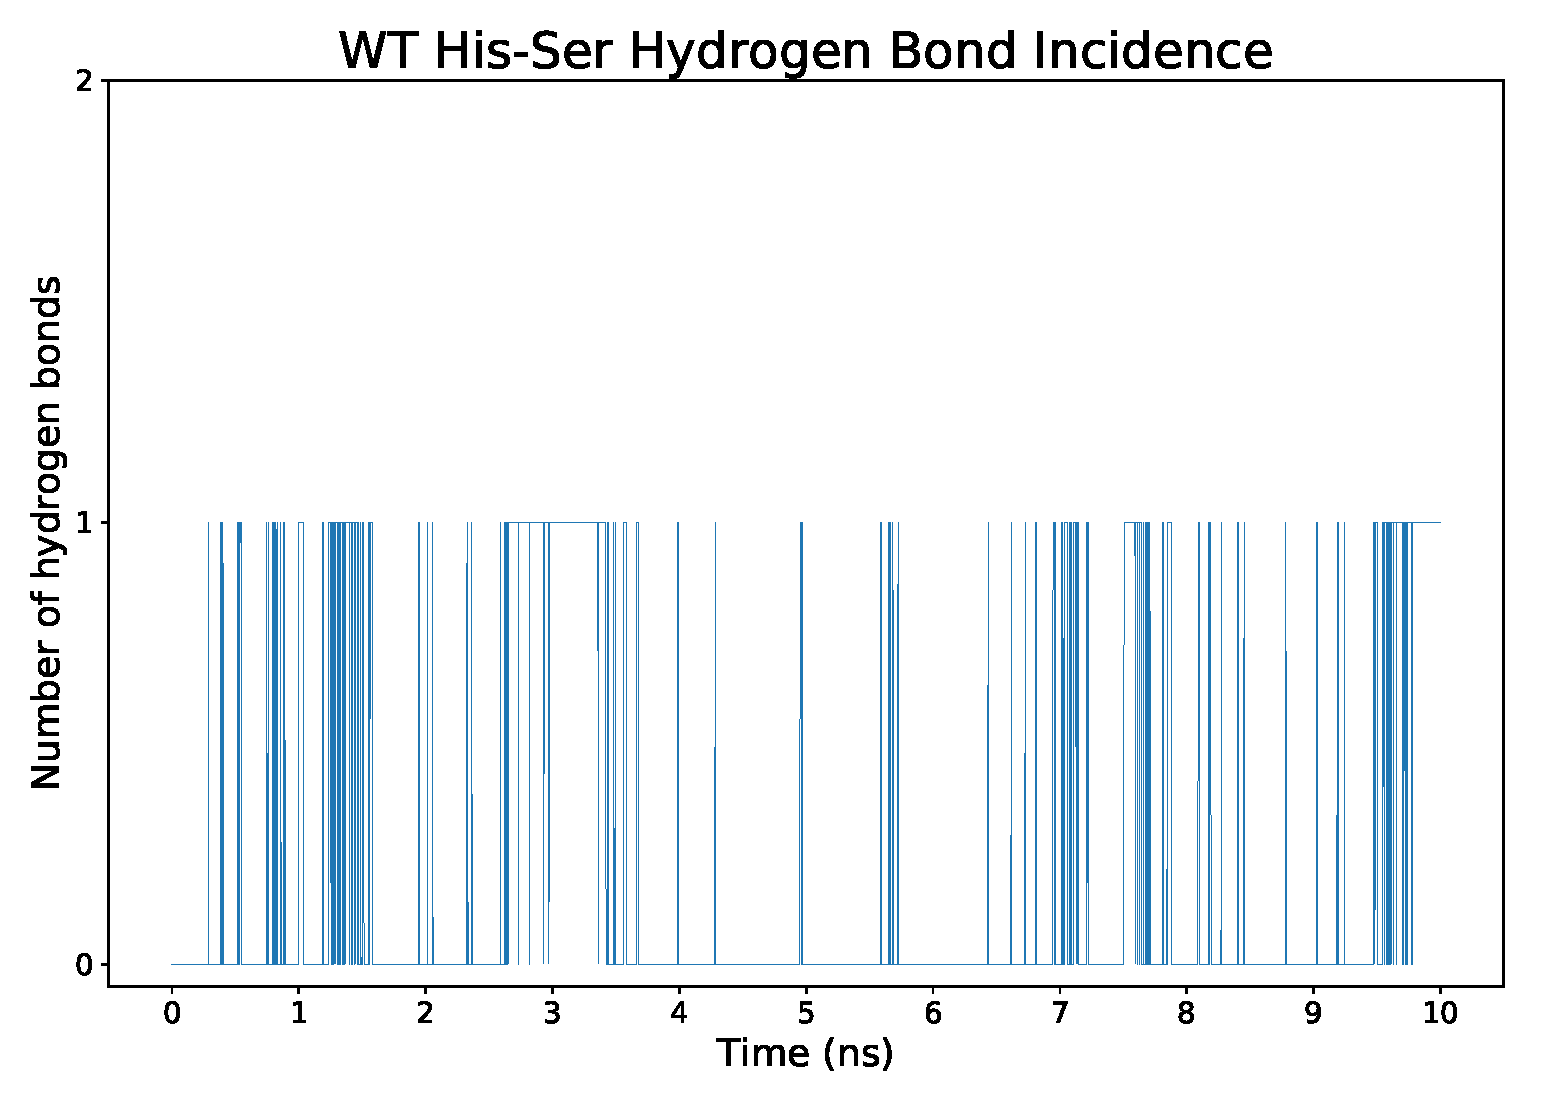
\includegraphics[width=0.49\textwidth]{wt_hbonds_his_ser.eps}
    \caption{}
\end{figure}

\begin{figure}[H]
    \centering
        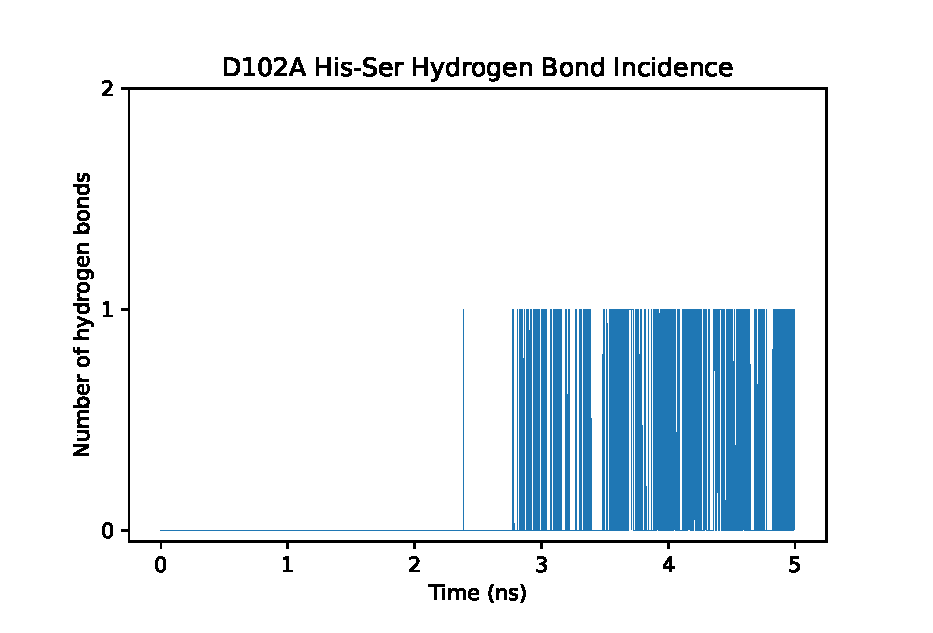
\includegraphics[width=0.49\textwidth]{d102a_hbonds_his_ser.eps}
    \caption{}
\end{figure}

\begin{figure}[H]
    \centering
        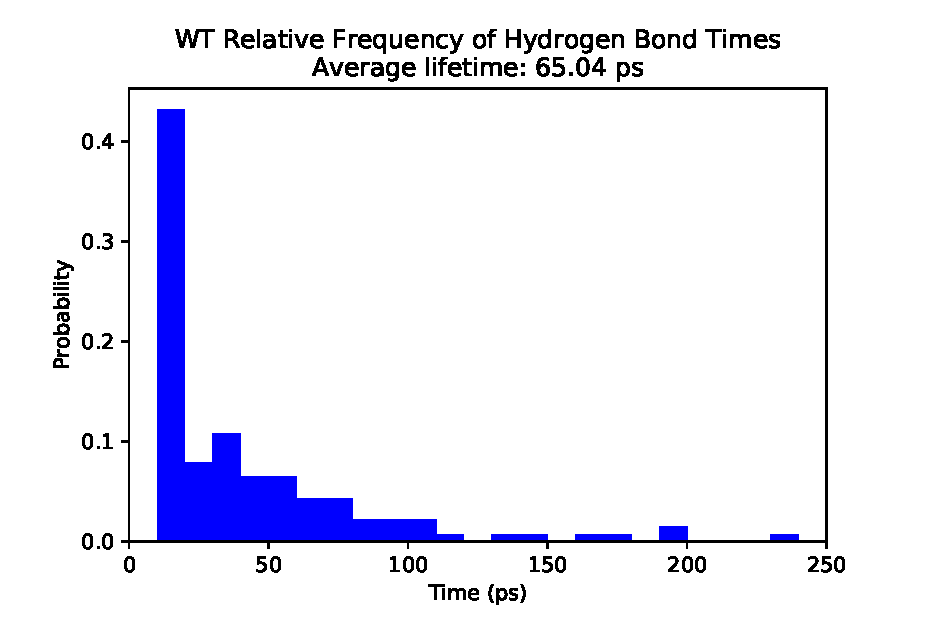
\includegraphics[width=0.49\textwidth]{wt_hbond_times.eps}
    \caption{}
\end{figure}

\begin{figure}[H]
    \centering
        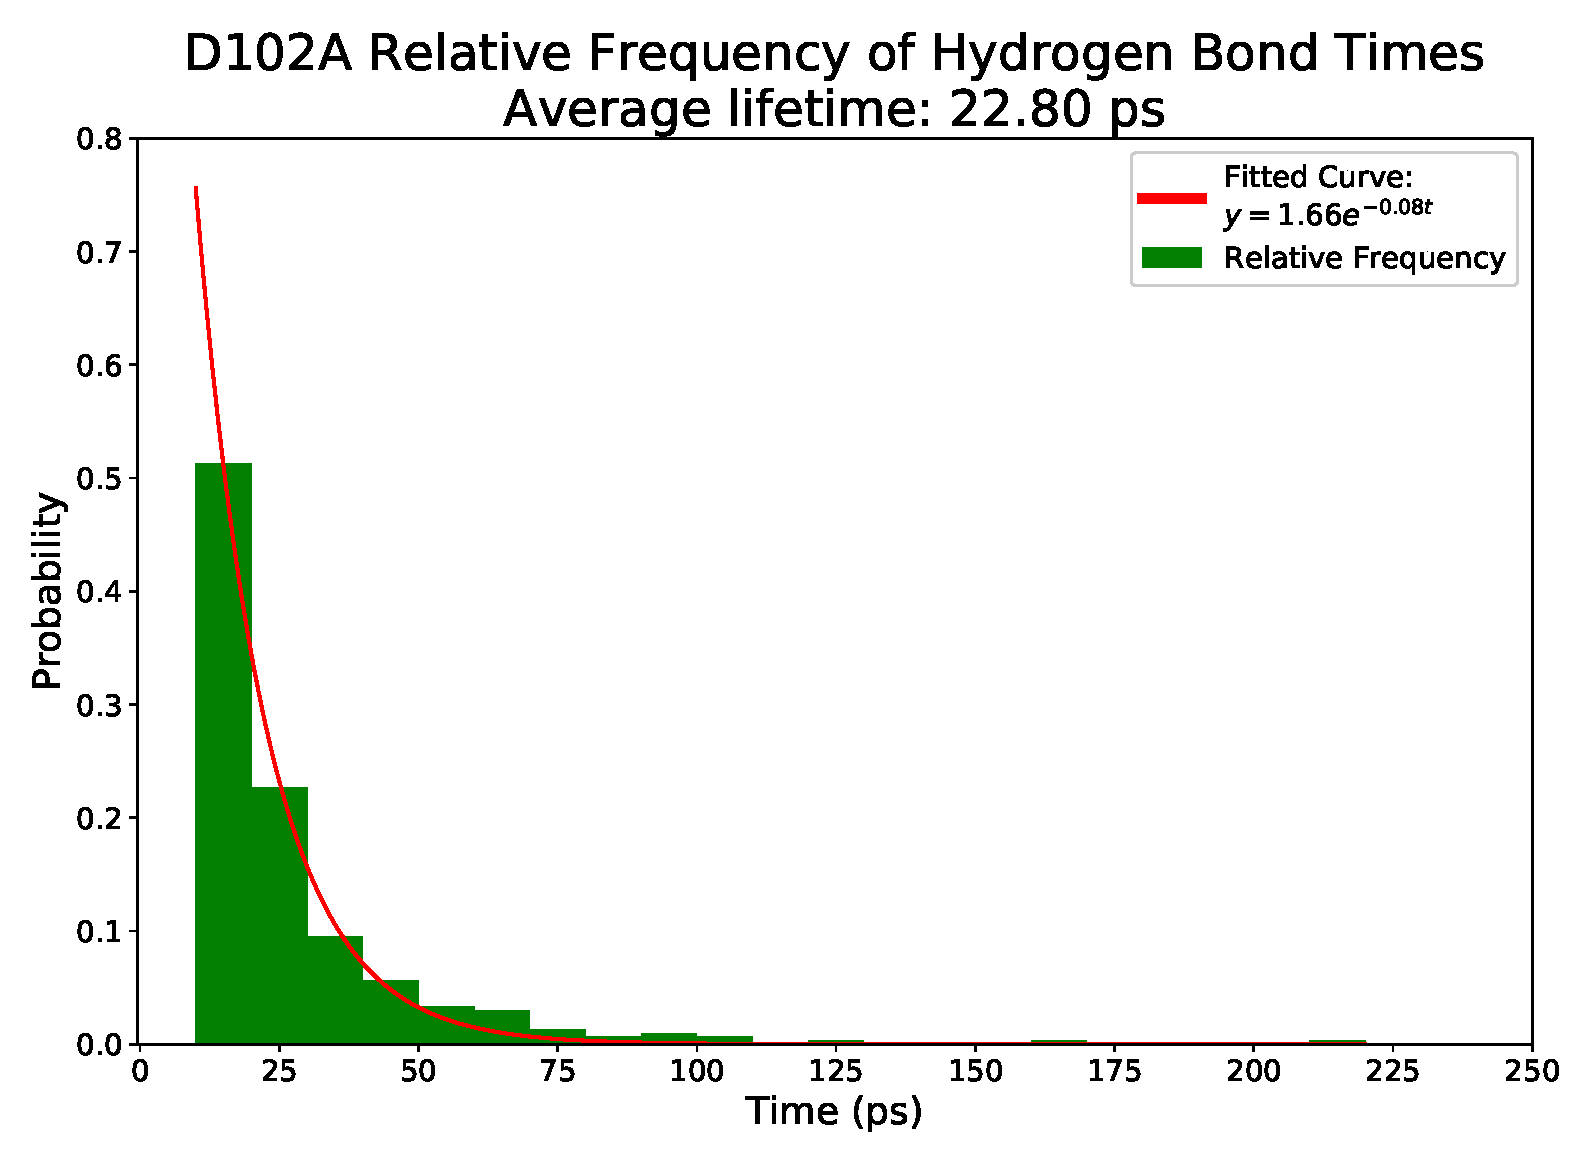
\includegraphics[width=0.49\textwidth]{d102a_hbond_times.eps}
    \caption{}
\end{figure}





\section{Conclusion}

\subsubsection*{Acknowledgements}

\section{References}
\begin{thebibliography}{9}
\bibitem{hedstrom02}
Hedstrom L. Serine protease mechanism and specificity.
Chemical reviews. 2002 Dec 11;102(12):4501-24.

\bibitem{madala10}
Madala PK, Tyndall JD, Nall T, Fairlie DP.
Update 1 of: Proteases universally recognize beta strands in their active sites.
Chemical reviews. 2011 Apr 8;110(6):PR1-31.


\end{thebibliography}

\appendix

\onecolumn

\section{Hydrogen Bond Lifetime Code}

Minted portion to be added later.

\end{document}